\subsection{The L-$z$ Plane}
Having obtained an as-near-to-homogenous set of photometry as we can, 
we are now in a position to calculate the Absolute Magnitudes of the VH$z$Q 
sample and in particulare the absolute magnitude at rest-frame 1450\AA\ , $M_{1450}$, 
which is a key physical quantity and goes directly towards the quasar luminosity 
function and thus the reionization of hydrogen calculation. 

We calculate the Distance Modulus in the normal fashion, 
\begin{equation}
m_{1450} - M_{1450} = 5 \log \left (    \frac{ D_{\rm L}(z)}{\rm Mpc}  \right )  + 25 + K_{\rm corr}(X,z)
\end{equation}
where $m_{1450}$ is the apparent magnitude at 1450\AA\ ,  
%$M_{1450}$ is the absolute magnitude at 1450 \AA\ , 
$D_{\rm L}(z)$ is the luminosity distance and 
$K_{\rm corr}(X,z)$ is the $K$-correction which corrects for the effects of redshifting of the bandpass and the spectrum. 

The $m_{1450}$ apparent magnitude is derived from the $z-$, $y/Y-$ or $J-$band photometery.

The Pan-STARSS1 $z_{\rm PS1}$ and $y_{\rm PS1}$-bands approximatley
sample the redshift ranges $4.53\leq z \leq 5.45$ and $5.28\leq z \leq 6.47$, respectively 
for 1450\AA'\ emission, while the VIRCAM $Y_{\rm VIRCAM}-$ and $J_{\rm VIRCAM}$-bands 
cover $5.50\leq z \leq 6.57$ and $7.06\leq z \leq 8.16$. 

\citet{Ross2013} has a detailed discussion of the $K$-correction (see that papers' Appendix B). 
The key result in that paper is, if quasars are described as having a power-law slope, 
$\alpha^{\nu}$ in spectral flux density, i.e., $f_\nu(\nu) \propto \nu^{\alpha_{\nu}}$ (as is conventional) 
then 
\begin{equation}
K_{\rm corr}(z) = -2.5 (1 + \alpha_{\nu}) \log[1 + z].
\end{equation}
Here the $[-2.5 \log(1 + z)]$ term corrects for the effective narrowing of the filter width with redshift, (the ``bandpass correction'') and the $[-2.5 \alpha^{\nu} \log(1 + z)]$ term takes into account the spectral index correction. The bandpass correction is approximately $\approx -1.945$ at redshift $z=5$ decreasing to $-2.32$ at redshift $z=7.50$. 


%At $z=5.00$, the rest-frame 1450\AA\ emission is redshifted to 8700\AA\ observed, i.e., in the $z$-band, while at $z=6.00$, $z=5.00$


\begin{figure*}
  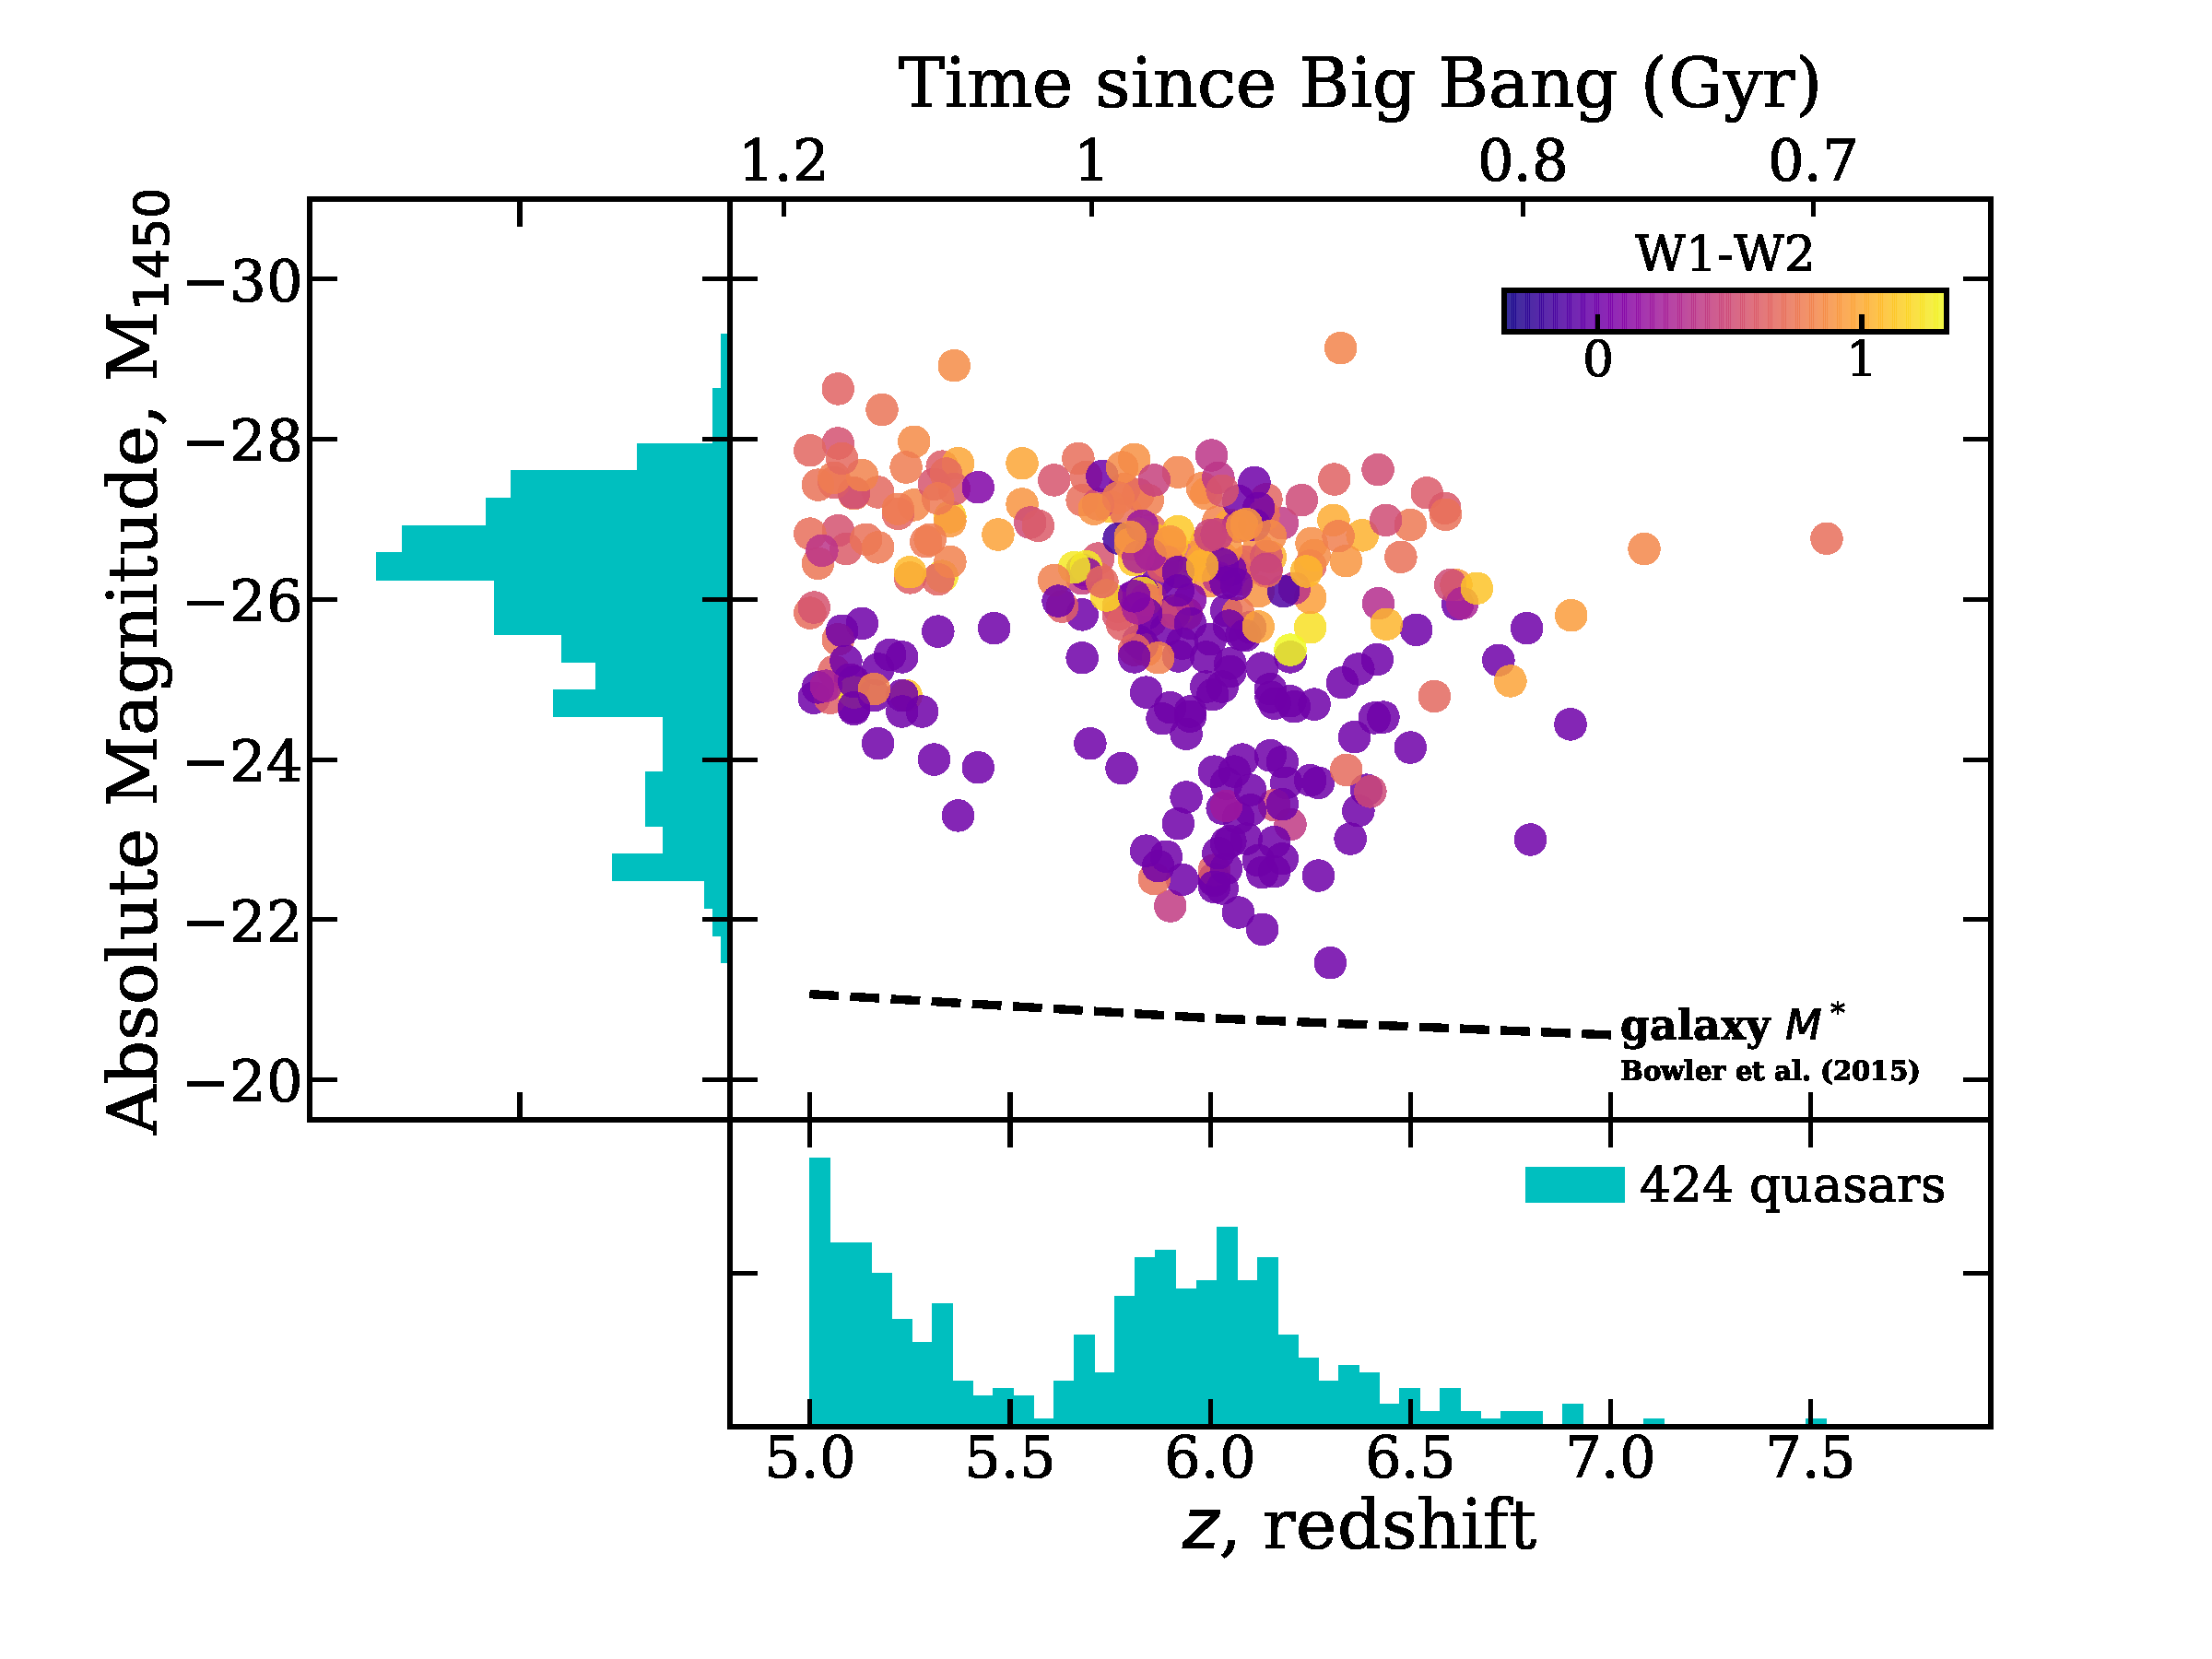
\includegraphics[width=18.0cm]
  {/cos_pc19a_npr/programs/quasars/highest_z/Lz/VHzQ_Lz_20180702.pdf}
  \centering
  \caption[]
  {The spectral bands used by different survey telescopes and that are relevant here.}
  \label{fig:Lz}
\end{figure*}
